\section{Cache misses, Branch mispredictions and Translation Lookaside Buffer misses}

\subsection{Cache misses}
A cache is a small fast memory storage that holds the most recently used memory words.
Caches improves on the memory latency so memory access can be achieved within the demand of modern processors.
Modern memory systems usually have three cache: Level 1 (L1), Level 2 (L2) and Level 3 (L3). 

\begin{figure}
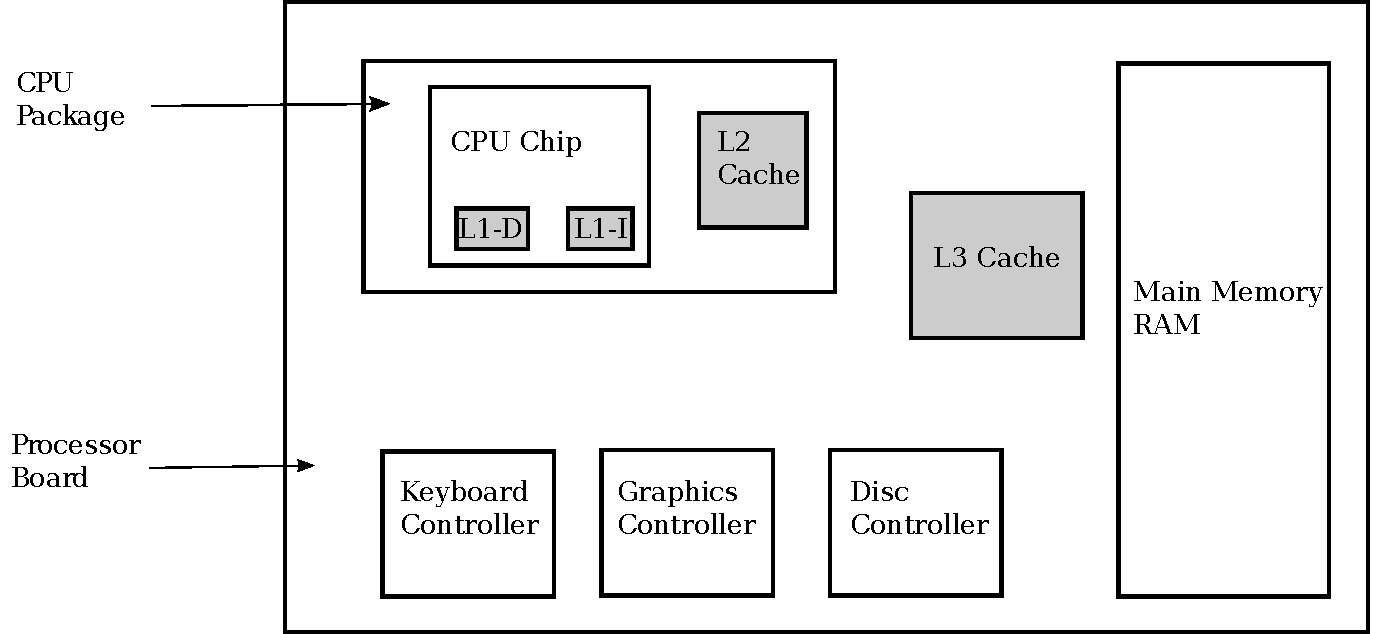
\includegraphics[width=\textwidth]{CacheLevels.pdf}
\end{figure}



The L1 cache resides on the CPU chip itself and usually has a size in the range from 16 KB to 128 KB and because it is placed directly on the CPU chip it is able to provide very fast memory access.

The L2 cache is placed next to the CPU chit and connected to it via a high speed path. It typically has a size between 512 KB and 1 MB which means that it can hold more data but is not able to provide as fast access as L1.

The L3 cache is placed on the processor board and usually has a size around 3 MB. Since it is placed further away from the cpu it is not able to provide as fast access as L1 and L2 but still much faster than fetching data from RAM.




\subsection{Branch Mispredictions}

\subsection{Translation Lookaside Buffer misses}

\section{Notes on Implementation}

\subsection{Machines used}
[Specs of all machines used for testing]

Machine 1: Jan's ASUS
Machine 2: Roland's ASUS

\subsection{Using Integers as Characters}
\label{sec:UsingIntAsChar}
The Wavelet Tree is a data structure for strings. 
Using the C++ \texttt{char array} or C++11 \texttt{string} types would seem natural in this case, but they each have problems.
The C and C++ \texttt{char} type is only of size 1 byte allowing us only to use an alphabet size of up to 256, making testing the running times dependency on alphabet size near-impossible as inaccuracies in the running time would likely exceed the difference in running time between the available sizes of the alphabet.

The C++11 \texttt{string} and arrays of type \texttt{char32\_t} doesn't have this problem and supports character types up to 32-bit unsigned. 
The problem lies in output and readability as characters corresponding to byte values below 32 are special non-printable control characters such as carriage-return and backspace. 
At higher byte values, other non-printable control characters and otherwise unreadable characters appear again, it means we would have to be very selective with the allowed byte values in our alphabets if we want it to be readable for output and debugging, and likely end up with an alphabet that is non-continuous on the set of byte values as a result.
Because of this, we have for convenience chosen to simply use arrays of integers as our strings in our implementations.
This will have no impact on performance as both characters and integers are simply different representations of byte values, so.

We assume in our implementation that the alphabet is always continuous on the set of byte values and store the alphabet as a minimum and maximum value, instead of storing each value in some data structure to pass around or point into.
This is for convenience as any other non-continuous alphabet could simply be mapped to a continuous run of byte values and used in the same way. 
This mapping could e.g. be done by storing an array of the alphabet in sorted order and using pointers into this array to signify the characters. 
Lookup into the array wouldn't be necessary unless printing for human reading as comparison of the pointer addresses will return same result as comparing the bytes.

We will still use the terms "character" and "string" in our descriptions of the algorithms even though we have implemented them as integers and integer arrays, as we feel the terms "character" and "string" are more intuitive and give clarity.


\subsection{Generating the Data}
We implemented a small script in Python to generate our input strings and write them in binary format to files.
This was slower than e.g. piping from \texttt{/dev/random} into a file, but we needed to constrain the alphabet and even though slow, a python script was the easiest way to achieve that.

\subsection{Reading Input}
At first we simply read from stdin using the \texttt{getline(cin, \&string)} function. 
Once we applied a profiler we found this to be horrendously slow, our Naïve algorithm spending about 20\% of its running time on resizing IO buffers. 
We then switched to using the \texttt{ifstream} class and IO time was reduced significantly to below 1\% of total running time.

\subsection{Verifying the Results}
To ensure that our implementations are correct, we implemented some simple and slow algorithms in python to calculate rank and select on the same input data we construct the wavelet trees on.
The point being that the python implementation should be so simple and easy to understand that it would be extremely unlikely to be wrong.
We then compare results from rank and select queries on our wavelet tree to results from the same queries using the python implementation.
When they agree on several randomly selected sets of query parameters, we feel confident our wavelet tree construction, rank, and select implementations are correct.

\subsection{Combating Over-Optimization}
The GNU Compiler Collection (GCC) is an optimizing compiler and can sometimes using static analysis recognize that the results and possible side-effects of a computation will not be used in the code and will in those cases completely remove that computation as an optimization.
This means that the compiler could potentially remove the entirety or parts of the computation for our queries when we test it, if we don't use the result for anything.
To ensure that the compiler doesn't throw needed computations out the window in our tests, we collect the results of each query in an array and print it to stdout. We only print it after the collection of measurements is done so as to effect the running time minimally.

\subsection{Reducing Construction Time Memory Usage}
Since the Wavelet tree is a recursively defined data structure, we also implement it recursively. 
Since it is also binary (or $d$-ary) we recurse into several sub-node constructors in the construction of a node, which means our compiler can't do tail-recursion optimisation \textbf{[TODO: check that this is true!]}. 
This further causes any stack-allocated variables to be held in memory until we leave the scope of the constructor function.
We traverse and split the input string into its left and right parts in each node constructor and thus end up holding the input string twice in memory: once in the variable holding the input string, once in the two variables holding the left and right split strings.
This is wasted memory because we don't actually need the input string any longer once we have split it into its left and right parts.
Because we simply call one sub-node constructor, then the other, once the first has completed, and finally return once both subnodes has completed constructing themselves, we end up completing the construction of the nodes in post-order.
This means we will keep the scopes of the root node, and those near the root, alive for most of the running time of the construction algorithm, and much memory is wasted.
The solution is to allocate these strings on the heap instead, passing pointers to the subnode constructors and having them delete them (as their input strings) once they have split them.
Doing this reduced the memory usage so much that we could run it for input strings with a length above $10^8$ without exhausting the about 6GB available memory on machine 1.


\subsection{Bitmap implementation choice}
There are several bitmap implementations available to us. In the STL there is \texttt{std::bitset<size\_t N>} and \texttt{std::vector<bool>}. From the Boost library there is \texttt{boost::dynamic\_bitset<>}.
\begin{description}
\item[\texttt{std::bitset}] While it would technically be possible to use the \texttt{std::bitset}, it requires that the size of the bitset is known at compile time and passed as a template parameter. This means we would need to recompile the program for each $n$, or size of the input string. 
We would also need to allocate a bitmap with room for $n$ bits for each sub-node as that is the theoretically possible size required, making the size required for the bitmaps of the tree $O(n \times |nodes|) = O(n2^{log(\sigma)})$ instead of $O(n \times height) = O(n~log(\sigma))$.
In the preallocated implementation of the Wavelet Tree we cannot use \texttt{std::bitset} either since it does not support pointer access, which means that we cannot do queries using \texttt{popcount}.
We also feel that an actual usable practical implementation should be able to handle different sizes of input at runtime instead of compile-time. 

\item[\texttt{boost::dynamic\_bitset}] is the Boost library's take on a dynamic bitset. 
It doesn't try to mimic a container and lacks some features such as an iterator because of that. 
It also does not guarantee that the bits will be allocated consecutively in memory and has no raw pointer access to the data in memory. 
This is a problem when we want to call popcount on all machine words from beginning up to some index.

\item[\texttt{vector<bool>}] is a specialised implementation for \texttt{bool} that packs the data so that each \texttt{bool} only takes up one bit and is not an actual C++ container, though it tries to mimic some of the behaviour. 
It is basically the STL implementation of a dynamically allocated bitset. This is the implementation we decided to use for our bitmap because it allows dynamic allocation and pointer access.
\end{description}

